\documentclass[10pt,twocolumn,letterpaper]{article}

\usepackage{cvpr}
\usepackage{times}
\usepackage{epsfig}
\usepackage{graphicx}
\usepackage{amsmath}
\usepackage{amssymb}
\usepackage{gensymb}

% Include other packages here, before hyperref.

% If you comment hyperref and then uncomment it, you should delete
% egpaper.aux before re-running latex.  (Or just hit 'q' on the first latex
% run, let it finish, and you should be clear).
%\usepackage[pagebackref=true,breaklinks=true,letterpaper=true,colorlinks,bookmarks=false]{hyperref}

\cvprfinalcopy % *** Uncomment this line for the final submission

\def\cvprPaperID{****} % *** Enter the 3DV Paper ID here
\def\httilde{\mbox{\tt\raisebox{-.5ex}{\symbol{126}}}}

% Pages are numbered in submission mode, and unnumbered in camera-ready
%\ifcvprfinal\pagestyle{empty}\fi
\setcounter{page}{4321}
\begin{document}

%%%%%%%%% TITLE
\title{Omni-directional stereo for 360$\degree$ 3D virual reality video}

\author{First Author\\
Institution1\\
Institution1 address\\
{\tt\small firstauthor@i1.org}
% For a paper whose authors are all at the same institution,
% omit the following lines up until the closing ``}''.
% Additional authors and addresses can be added with ``\and'',
% just like the second author.
% To save space, use either the email address or home page, not both
\and
Second Author\\
Institution2\\
First line of institution2 address\\
{\tt\small secondauthor@i2.org}
}

\maketitle
%\thispagestyle{empty}

%%%%%%%%% ABSTRACT
\begin{abstract}
   The aim of our project is to produce omni-directional stereo images and videos, which are for example viewable in the Google Cardboard. The input for our pipeline are the images of a camera rig, which are stitched together for receiving omni-directional images. This process has to been carried out twice, once for the left and once for the right eye to get an omni-directional stereo image.
\end{abstract}

%%%%%%%%% BODY TEXT
\section{Introduction}

The stereo view of our eyes is created by fusing the image from the left eye with the one from the right eye. This enables us to perceive a stereo impression of the world. Therefore, to produce stereo videos, we need to capture synchronized videos from two cameras set apart at interpupillary distance (IPD), which denotes the distance between the two eyes and is on average about 6.4 cm. However, the goal of this project is not only to produce stereo, but omni-directional, which means 360$\degree$, videos. The first simple idea coming in mind to capture such videos is to place two omni-directional cameras with a distance of IPD. One issue with such an approach is that the two cameras will see each other, which is undesirable. However, the more important problem is that objects lying on the line between the two camera centers will have no disparity (see figure 1). Disparity denotes the amount of shift in the image position between the left and the right eye. Therefore, this simple solution does not work and would not produce the desired omni-directional stereo videos.

The ideal solution would be to have a stereo image pair for every head orientation, for example one pair for each degree (see figure 2). However, this would be a huge amount of images. The main idea is to approximate this optimal view by only capturing the central ray of each camera instead of the full image at each head orientation (see figure 3).

\begin{figure}[t]
\begin{center}
\fbox{\rule{0pt}{2in} \rule{0.9\linewidth}{0pt}}
   %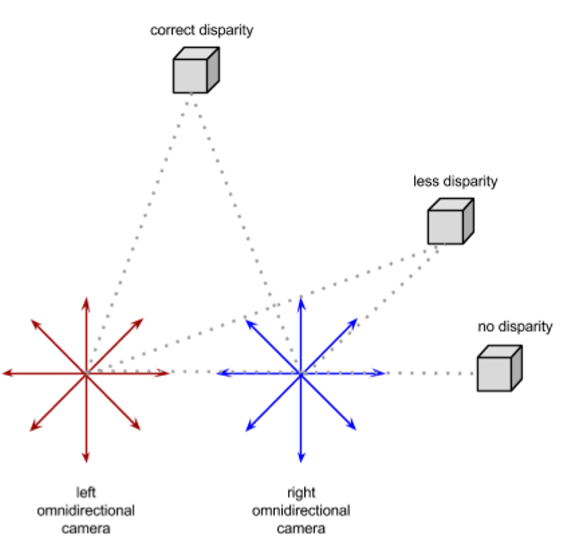
\includegraphics[width=0.8\linewidth]{/pictures/two_360.png}
\end{center}
   \caption{Illustration of two 360$\degree$ cameras placed next to each other.}
\label{fig:long}
\label{fig:onecol}
\end{figure}

\begin{figure}[t]
\begin{center}
\fbox{\rule{0pt}{2in} \rule{0.9\linewidth}{0pt}}
   %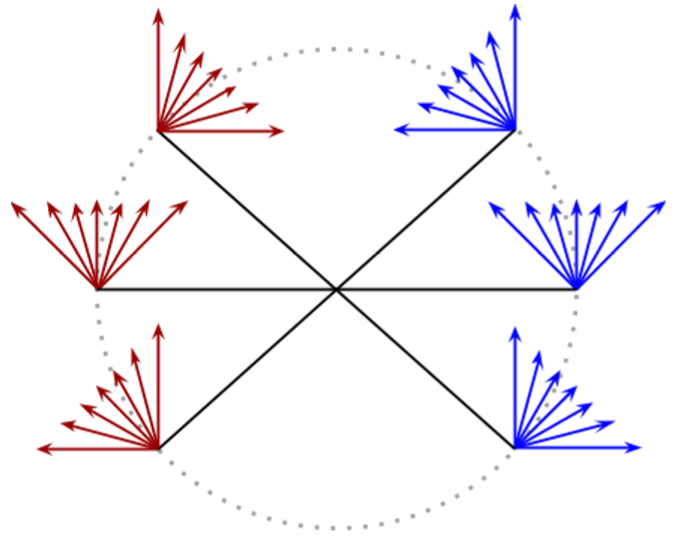
\includegraphics[width=0.8\linewidth]{/pictures/wanted.png}
\end{center}
   \caption{This image shows the most optimal situation, where a full image is captured for each head direction. The red rays illustrate the left eye and the blue ones the left eye.}
\label{fig:long}
\label{fig:onecol}
\end{figure}

\begin{figure}[t]
\begin{center}
\fbox{\rule{0pt}{2in} \rule{0.9\linewidth}{0pt}}
   %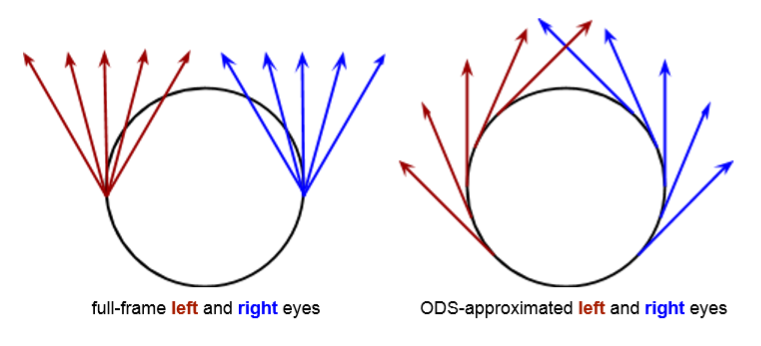
\includegraphics[width=0.8\linewidth]{/pictures/approxi.png}
\end{center}
   \caption{The left image shows the rays for capturing the full image at one head direction. The right image illustrates the ODS approximation by using only the central ray of each camera position.}
\label{fig:long}
\label{fig:onecol}
\end{figure}


%------------------------------------------------------------------------
\section{Related work}


%------------------------------------------------------------------------
\section{Method}



%------------------------------------------------------------------------
\section{Results}


%------------------------------------------------------------------------
\section{Discussion}


%------------------------------------------------------------------------
\section{Conclusion}







{\small
\bibliographystyle{ieee}
\bibliography{egbib}
}

\end{document}
